\documentclass[b4paper, landscape, dvipdfmx]{jsarticle}
%----- 必要なパッケージ -----
\usepackage{fancybox,ascmac,otf,ulem}
\usepackage{amssymb, amsthm}
\usepackage[leqno]{amsmath}
\usepackage{wrapfig}
\usepackage{geometry}
\usepackage{multicol}
\usepackage{tcolorbox}
\usepackage{xcolor}
\usepackage{fancyhdr}
\usepackage{tikz}

% shadowsライブラリ
\usetikzlibrary{
    positioning,
    arrows.meta,
    calc,
    shadows,
    shadows.blur,
    intersections
}

\tcbuselibrary{skins, breakable, theorems}
\usepackage{enumitem}
\setlist[enumerate,1]{label=(\arabic*)}
\setlist[itemize]{leftmargin=*}
\newcommand{\ds}{\displaystyle}

%----- レイアウト設定 -----
\geometry{
  left=15mm,
  right=15mm,
  top=20mm,
  bottom=15mm,
  headheight=25pt
}

%----- 数式環境の上下の余白調整 -----
\AtBeginDocument{
  \setlength{\abovedisplayskip}{5pt}
  \setlength{\belowdisplayskip}{5pt}
  \setlength{\abovedisplayshortskip}{0pt}
  \setlength{\belowdisplayshortskip}{3pt}
}

%===========================================================
%  デザイン設定
%===========================================================

%--- 色の定義 ---
\definecolor{printBlue}{RGB}{0, 50, 100}     % 濃紺
\definecolor{printRed}{RGB}{140, 20, 20}     % 濃エンジ
\definecolor{printTeal}{RGB}{0, 60, 60}      % 濃い青緑
\definecolor{gridColor}{gray}{0.75}          % 解答欄の方眼

%--- 共通スタイル定義 ---
\tcbset{
    chartbox/.style={
        enhanced,
        fonttitle=\sffamily\bfseries,
        boxrule=1pt,
        arc=2pt,
        top=1.0em,
        nobeforeafter,
        enlarge left by=-2mm,
        enlarge right by=-2mm,
        drop fuzzy shadow,
        colback=white,
        attach boxed title to top left={xshift=10pt, yshift*=-\tcboxedtitleheight/2},
        boxed title style={frame hidden, sharp corners, rounded corners=southeast, arc=3pt}
    }
}

% 各種ボックス環境定義
\newenvironment{overall}[1]{
\begin{tcolorbox}[
    chartbox,
    colframe=printTeal,
    coltitle=white,
    title=\textbf{全体課題 #1},
    boxed title style={colback=printTeal},
]}
{\end{tcolorbox}}

\newtcolorbox{any}[1]{
    enlarge left by=0mm, enlarge right by=0mm,
    enhanced, frame hidden, colback=white, title={#1},
    attach boxed title to top left={xshift=0mm, yshift=0mm},
    coltitle=white, fonttitle=\bfseries\sffamily,
    boxed title style={
        colback=black!80, frame hidden, arc=4pt, outer arc=4pt,
        sharp corners=south, boxrule=0pt,
        top=1mm, bottom=1mm, left=3mm, right=3mm
    },
    underlay boxed title={
        \draw[thick, black!80] (title.south west) -- (title.south west-|frame.east);
    },
    breakable, top=5mm, left=2mm, right=2mm, bottom=0mm,
    before skip=1em, after skip=1em,
    segmentation style={draw=black!40, dashed}
}


\newenvironment{eg}[1]{
\begin{tcolorbox}[
    chartbox,
    colframe=printBlue,
    coltitle=white,
    title=\textbf{例題 #1},
    boxed title style={colback=printBlue},
    segmentation style={draw=printBlue, line width=0.5pt, dashed}
]}
{\end{tcolorbox}}

\newenvironment{prac}[1]{
\begin{tcolorbox}[
    chartbox,
    colframe=printRed,
    coltitle=white,
    title=\textbf{練習 #1},
    boxed title style={colback=printRed}
]}
{\end{tcolorbox}}

\newenvironment{answer}[1][height fill]{
    \begin{tcolorbox}[
        enhanced,
        title={Memo / Answer},
        colframe=black!80,
        colback=white,
        coltitle=black!60,
        fonttitle=\sffamily\bfseries,
        attach boxed title to top left={xshift=5mm, yshift*=-\tcboxedtitleheight/2},
        boxed title style={frame hidden, colback=white},
        boxrule=1pt,
        arc=1pt,
        nobeforeafter,
        enlarge left by=2mm, 
        enlarge right by=2mm, 
        height fill,
        segmentation style={draw=black!20, solid},
        underlay={
            \begin{tcbclipinterior}
                \draw[step=5mm, black!5, ultra thin] (interior.south west) grid (interior.north east);
            \end{tcbclipinterior}
        }, 
        #1
    ]}
{ \end{tcolorbox}}

%----- 段組の設定 -----
\setlength{\columnsep}{15mm}
\setlength{\columnseprule}{0.4pt}
\renewcommand{\columnseprulecolor}{\color{black!30}}

%----- ヘッダーの設定 -----
\pagestyle{fancy}
\fancyhf{}

% ヘッダーデザイン
\fancyhead[C]{%
    \begin{tikzpicture}[remember picture, overlay]
        \node[anchor=north west, fill=printBlue, minimum width=\paperwidth, minimum height=5pt] at (current page.north west) {};
    \end{tikzpicture}
}
\fancyhead[L]{\small \textcolor{black!90}{数学\ajRoman{2} $>$ 第2章 複素数と方程式 $>$ 第8回--\textbf{方程式とグラフ}}}
\fancyhead[R]{\small 年 \hspace{1cm} 組 \hspace{1cm} 番 \quad 氏名 \hspace{6cm}}
\renewcommand{\headrulewidth}{0pt}

\begin{document}

\begin{multicols*}{2}

%===========================================================
% 左カラム: 実数解と共有点
%===========================================================

{\large \textbf{1. 方程式の解 $\iff$ グラフの共有点}}

\begin{any}{「解く」ことの図形的意味}
方程式 $P(x)=0$ の\textbf{実数解}は, グラフ $y=P(x)$ と $x$軸(直線 $y=0$)との\textbf{共有点の $x$座標}と一致する.

\begin{center}
    \begin{tikzpicture}[scale=0.8]
        \draw[->, >=stealth] (-1.5,0) -- (3.5,0) node[right] {$x$};
        \draw[->, >=stealth] (0,-1.5) -- (0,2) node[above] {$y$};
        % 3次関数のグラフ
        \draw[thick, domain=-1.2:3.2, smooth, variable=\x, blue] plot ({\x}, {0.3*(\x+1)*(\x-1)*(\x-3)});
        
        \fill[red] (-1,0) circle (2pt) node[above left] {$\alpha$};
        \fill[red] (1,0) circle (2pt) node[above right] {$\beta$};
        \fill[red] (3,0) circle (2pt) node[above right] {$\gamma$};
        
        \node[blue] at (2, 1.5) {$y=P(x)$};
        \node[red, align=left] at (1, -1.8) {方程式 $P(x)=0$ の実数解は\\グラフの $x$ 切片!};
    \end{tikzpicture}
\end{center}

つまり, 方程式を解くことは, グラフがどこで $x$軸と交わるかを探すことと同じである.
\end{any}

\begin{eg}{1(共有点の座標)}
次の3次方程式を解き, グラフ $y=x^3-4x^2+x+6$ と $x$軸の共有点の座標をすべて求めよ.
\[ x^3 - 4x^2 + x + 6 = 0 \]
\end{eg}

\begin{answer}

\end{answer}

\columnbreak

%===========================================================
% 右カラム: 重解と接点
%===========================================================

{\large \textbf{2. 重解 $\iff$ 接点}}

\begin{any}{接することの条件}
方程式が\textbf{重解}をもつとき, グラフは $x$軸と\textbf{接する}.
\begin{itemize}
    \item $(x-\alpha)^2$ を因数にもつ $\to$ $x=\alpha$ で $x$軸に接する.
    \item $(x-\alpha)^3$ を因数にもつ $\to$ $x=\alpha$ で接しながら突き抜ける(3重解).
\end{itemize}
\end{any}

\begin{eg}{2(重解をもつケース)}
方程式 $x^3 - 3x + 2 = 0$ を解き, グラフと $x$軸の共有点の座標を求めよ. また, 接点の $x$座標を答えよ.
\end{eg}

\begin{answer}[height=10cm]

\end{answer}

\begin{any}{虚数解の図形的意味}
方程式 $x^3-1=0$ の解は $x=1, \frac{-1\pm\sqrt{3}i}{2}$ であった.
実数解は「1」だけである.
これは, グラフ $y=x^3-1$ が \textbf{$x$軸と1か所 ($x=1$) でしか交わらない} ことを意味している.
(虚数解はグラフ上には見えない!)
\end{any}

\end{multicols*}

\newpage

%===========================================================
% 裏面: 演習問題
%===========================================================

\begin{multicols*}{2}

{\large \textbf{確認テスト}}

\begin{prac}{A1(共有点探し)}
次の方程式を解き, グラフ $y=P(x)$ と $x$軸の共有点の座標をすべて求めよ.
\begin{enumerate}
    \item $x^3 - 2x^2 - 5x + 6 = 0$
    \item $x^3 + 3x^2 - 4 = 0$
\end{enumerate}
\end{prac}


\begin{prac}{A2(グラフから式を読み取る)}
右の図は, ある3次関数 $y=P(x)$ のグラフである.
このグラフから読み取れる方程式 $P(x)=0$ の解をすべて答えよ.
また, 重解となっているものはどれか.
\begin{center}
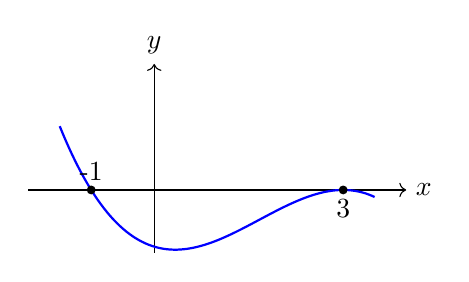
\begin{tikzpicture}[scale=0.8]
    \draw[->] (-2,0) -- (4,0) node[right] {$x$};
    \draw[->] (0,-1) -- (0,2) node[above] {$y$};
    % x=-1で交わり, x=3で接するグラフ
    \draw[blue, thick, smooth, samples=100, domain=-1.5:3.5] plot (\x, {-0.1*(\x+1)*(\x-3)*(\x-3)});
    \fill[black] (-1,0) circle (2pt) node[above] {-1};
    \fill[black] (3,0) circle (2pt) node[below] {3};
\end{tikzpicture}
\end{center}
\end{prac}

\begin{answer}
% 解: x = -1, 3
% 重解: x = 3 (接しているから)
\vspace{3cm}
\end{answer}

\columnbreak

\begin{prac}{B1(解の個数とグラフ)}
3次方程式 $x^3 - 3x^2 + 4 = 0$ について以下の問いに答えよ.
\begin{enumerate}
    \item 方程式の実数解を求めよ.
    \item グラフ $y=x^3-3x^2+4$ の概形として正しいものを次から選べ.
\end{enumerate}
\begin{center}
    (ア) \tikz[scale=0.3]{\draw[->](-2,0)--(2,0);\draw[blue] plot[domain=-1.5:1.5] (\x,{\x*\x*\x});} \quad
    (イ) \tikz[scale=0.3]{\draw[->](-2,0)--(3,0);\draw[blue] plot[domain=-1:2.5] (\x,{(\x+1)*(\x-2)*(\x-2)});} \quad
    (ウ) \tikz[scale=0.3]{\draw[->](-2,0)--(3,0);\draw[blue] plot[domain=-1:2.5] (\x,{(\x+1)*(\x-1)*(\x-2)});}
\end{center}
\end{prac}

\begin{prac}{B2(発展:実数解の個数)}
$k$ を定数とする. 3次方程式 $x^3 - 3x + k = 0$ が異なる3つの実数解をもつための条件を, グラフの平行移動をイメージして考察せよ.
(ヒント: $y=x^3-3x$ と 直線 $y=-k$ の共有点を考える)
\end{prac}

\begin{answer}
\end{answer}

\end{multicols*}

\end{document}